\subsubsection{Q10.20 data 09202021 10082021 grouped by scenario \& PGM}

\begin{comment}
                             EFPR        EO      EFNR     n    pvalue
(frauth, Advantaged)     0.543478  0.456522  0.478261  23.0  0.461535
(frauth, Disadvantaged)  0.409091  0.590909  0.545455  11.0  0.368024
(icu, Advantaged)        0.527778  0.472222  0.555556  18.0  0.944655
(icu, Disadvantaged)     0.450000  0.550000  0.700000  10.0  0.916512
(rent, Advantaged)       0.555556  0.444444  0.416667  18.0  0.518719
(rent, Disadvantaged)    0.433333  0.566667  0.333333  15.0  0.538385
\end{comment}

\begin{table}[h]
    \centering
    \begin{tabular}{|c|c|c|c|c|c|c|}
        \hline
        scenario & PGM & EFPR & EO & EFNR & n & p-value\\
        \hline
        frauth & Advantaged & \textbf{0.543} & 0.457 & 0.478 & 23.0 & 0.462\\
		frauth & Disadvantaged & 0.409 & \textbf{0.591} & \textbf{0.545} & 11.0 & 0.368\\
		icu & Advantaged & \textbf{0.528} & 0.472 & \textbf{0.556} & 18.0 & 0.945\\
		icu & Disadvantaged & 0.450 & \textbf{0.550} & \textbf{0.700} & 10.0 & 0.917\\
		rent & Advantaged & \textbf{0.556} & 0.444 & 0.417 & 18.0 & 0.519\\
		rent & Disadvantaged & 0.433 & \textbf{0.567} & 0.333 & 15.0 & 0.538\\
		
        \hline
    \end{tabular}
    \caption{Grouped by scenario PGM}
    \label{tab:my_label}
\end{table}
\begin{figure}[h]
    \centering
    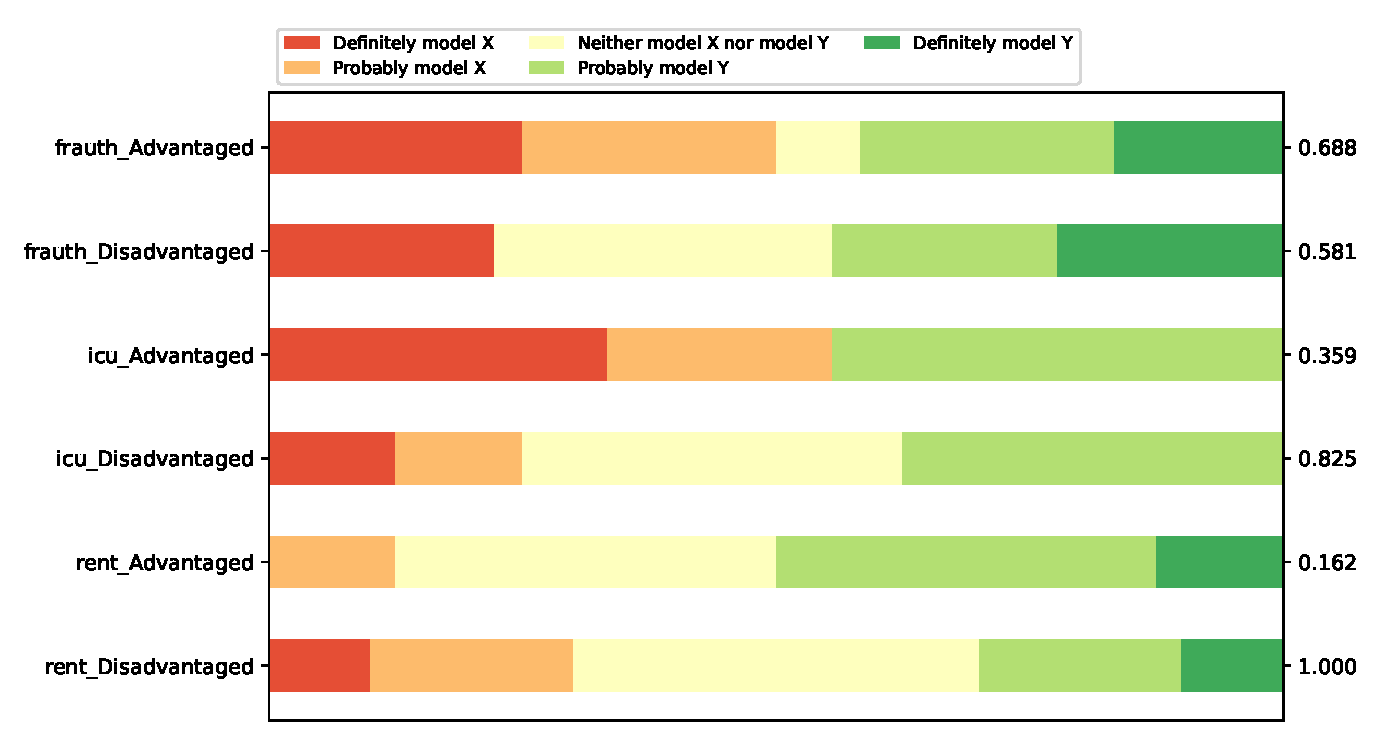
\includegraphics[width=0.8\textwidth]{figures/Q10.20/09202021_10082021/Q10.20_scenario_PGM.pdf}
    \caption{Grouped by scenario \& PGM}
    \label{fig:my_label}
\end{figure}
